\documentclass[11pt,a4paper]{article}
\usepackage[margin=2.5cm]{geometry}
\usepackage[T1]{fontenc}
\usepackage{lmodern,microtype,booktabs,graphicx,amsmath,siunitx,hyperref,caption}
\sisetup{scientific-notation=true,round-mode=figures,round-precision=2}
\hypersetup{colorlinks=true,linkcolor=black,urlcolor=blue}
\title{Equivalence of the Caffe and PyTorch implementations\\of the LysoQuant 2D U-Net}
\author{Technical verification report}
\date{29 October 2026}
\begin{document}
\maketitle

\begin{abstract}
\noindent LysoQuant originally segmented lysosomes with a 2D U-Net trained and executed in the \texttt{caffe\_unet} framework (model \texttt{2D-7-16}). The server now runs a PyTorch re-implementation. I verify that the two are the same function: (i) the PyTorch module graph matches the Caffe \texttt{prototxt} layer by layer; (ii) all $\num[scientific-notation=false,round-mode=none]{124440467}$ parameters are bit-identical to those in the Caffe weight file; (iii) the forward pass agrees with an independent NumPy interpreter of the \texttt{prototxt} to $\sim10^{-14}$ in double precision and $\sim10^{-6}$ (relative) in single precision, on synthetic and on real microscopy data, with 100\% identical class decisions; (iv) on a real image, the segmentation produced by the server differs from the one produced by the original Caffe plugin in 118 of $\num[scientific-notation=false,round-mode=none]{5193841}$ pixels (99.998\% identical; Dice $>0.9999$ for both classes), all at near-ties of the class scores on object borders. After excluding objects smaller than \SI{0.53}{\micro m\squared}, as the LysoQuant plugin does, the Caffe and PyTorch segmentations of this image contain exactly the same number of lysosomes (295 in total: 149 negative and 146 positive). In summary, the counts reported by LysoQuant are unaffected by the change of framework and segmentation masks have differences confined to single border pixels in undecided locations.
\end{abstract}

\section{Scope and method}
The question is whether \texttt{lysoquant-7-16.pt} (PyTorch, \texttt{server/lysoquant\_server/unet.py}) computes the same function as \texttt{2D-7-16.modeldef.h5} + \texttt{2D-7-16.caffemodel.h5} (Caffe). A U-Net is fully determined by (a) its computational graph, (b) its parameters, and (c) the exact semantics of each operator (padding, cropping, pooling, deconvolution layout). Each is checked separately, then jointly by running the networks on identical inputs.

To read the architecture and weights of the old network, I wrote a reference interpreter in plain NumPy (float64) that \emph{reads the \texttt{prototxt} embedded in the model file} and executes its test-phase layers in order, taking the weights of each layer by name from the Caffe HDF5 file. It shares no code with the PyTorch module nor with the converter (\texttt{convert.py}), so a mistake in the layer-name mapping, weight layout or crop logic of the port cannot be reproduced by the reference. All scripts are in \texttt{report/verification/}.

\section{Architecture}
The \texttt{prototxt} has 97 layers. Removing the training-only ones (HDF5 data, deformation, value augmentation, softmax loss; 7 layers) leaves the 90-layer test-time network (Table~\ref{tab:layers}). The model declares \texttt{num\_output: 16} base channels.

\begin{table}[h]\centering
\caption{Test-time layers of the Caffe network and their PyTorch counterparts.}\label{tab:layers}
\begin{tabular}{llr l}\toprule
Caffe layer & Parameters & Count & PyTorch\\\midrule
Convolution & $3{\times}3$, pad 0, stride 1 & 30 & \texttt{Conv2d(k=3)}\\
Convolution & $1{\times}1$ (score, 3 classes) & 1 & \texttt{Conv2d(k=1)}\\
Deconvolution & $2{\times}2$, stride 2, pad 0 & 7 & \texttt{ConvTranspose2d(2,2)}\\
ReLU & \texttt{negative\_slope: 0.1} (all 37) & 37 & \texttt{LeakyReLU(0.1)}\\
Pooling & MAX, $2{\times}2$, stride 2 & 7 & \texttt{max\_pool2d(2,2)}\\
Concat & [upsampled, encoder skip] & 7 & \texttt{torch.cat([up, crop(skip)])}\\
ValueTransformation & offset $-0.5$ & 1 & \texttt{x + (-0.5)}\\\bottomrule
\end{tabular}
\end{table}

For each of the 38 parameterised layers, in execution order, the script compares layer type, kernel size, stride, padding and output channels (and asserts that no \texttt{group}, \texttt{dilation} or \texttt{bias\_term} option is set) with the corresponding PyTorch module: all 38 match. The LeakyReLU slope is the single value $0.1$ in all 37 ReLU layers, which is the value used by the port, and PyTorch's \texttt{LeakyReLU} is $f(x)=x$ for $x>0$ and $0.1x$ otherwise, identical to Caffe's ReLU with \texttt{negative\_slope}. Note that the Caffe model applies an activation after the up-convolution but not after the final score layer; so does the port.

\paragraph{Operator semantics.} Caffe \texttt{Convolution} is a cross-correlation with weights shaped $(C_{out},C_{in},k_h,k_w)$, as in PyTorch. Caffe \texttt{Deconvolution} (the transpose of a convolution) stores weights as $(C_{in},C_{out},k_h,k_w)$, the layout of \texttt{ConvTranspose2d}; hence no transposition is needed. With $2{\times}2$ stride-2 kernels there is no overlap and the operation is a pixel-wise scatter (this is exactly how the NumPy reference implements it, independently of PyTorch). Caffe's pooling rounds output sizes up while PyTorch rounds down, but the two coincide whenever the feature map is even, which the server enforces by only using valid tile sizes.

\paragraph{Skip connections.} The $3{\times}3$ convolutions are unpadded, so encoder feature maps are larger than the up-sampled maps they are concatenated with. The \texttt{caffe\_unet} Concat layer centre-crops the larger blob; the port does the same (\texttt{\_center\_crop}). This is the one operator whose behaviour I take from the framework's documented behaviour rather than from the file; it is corroborated by the geometry below.

\section{Receptive-field geometry}
The model file stores \texttt{padInput}$=508$, \texttt{padOutput}$=-1020$, \texttt{downsampleFactor}$=128$, and the training layer uses $1788{\times}1788$ inputs. From the port's shape arithmetic: the smallest valid input is $1532$ (output $4$), valid sizes advance in steps of $128$, and every input is $1528$ px larger than its output. This agrees with the file: $508+1020=1528$, $128=2^7$, and $1788\to 260$ (since $260+1528=1788$). The $1528$ border decomposes as $4(2^7-1)=508$ for the encoder, $4\cdot2^7=512$ for the bottleneck and $508$ for the decoder; the stored \texttt{padInput}$=508$ is the encoder term. This is consistent with a symmetric centre-crop in the skip connections.

\section{Parameters}
The converter maps Caffe layer names to PyTorch parameters. To avoid trusting that mapping, the check pairs the 38 parameterised \texttt{prototxt} layers with the PyTorch modules \emph{by execution order} and compares tensors with \texttt{numpy.array\_equal}. Result: all 38 weight and 38 bias tensors are \textbf{bit-identical} ($\num[scientific-notation=false,round-mode=none]{124440467}$ parameters on both sides). The HDF5 file contains 105 entries under \texttt{/data}; 38 hold parameters, 8 are empty Caffe auto-inserted \texttt{*\_split} layers, and the remaining 59 are parameter-free layers (ReLU, pooling, concat, training-only layers). No weight in the file is left unused.

\section{Numerical equivalence of the forward pass}
\subsection{Reference test}
Random inputs were fed to (a) the NumPy \texttt{prototxt} interpreter in float64, (b) the PyTorch network in float64 and (c) in float32, using the smallest valid sizes ($1532$ and $1660$ px, outputs $4{\times}4$ and $132{\times}132$). Table~\ref{tab:synth} shows the maximum absolute difference against the reference.

\begin{table}[h]\centering
\caption{Synthetic inputs. Output scores have magnitude $\sim5$--$12$.}\label{tab:synth}
\begin{tabular}{llccc}\toprule
Input & Kind & PyTorch f64 & PyTorch f32 & argmax equal\\\midrule
1532 & uniform & \num{3.6e-15} & \num{6.0e-06} & 100\%\\
1532 & blobs+noise & \num{1.2e-14} & \num{7.7e-06} & 100\%\\
1660 & uniform & \num{3.5e-14} & \num{2.0e-05} & 100\%\\
1660 & blobs+noise & \num{3.2e-14} & \num{1.5e-05} & 100\%\\\bottomrule
\end{tabular}
\end{table}

In double precision the two programs agree to machine precision (round-off of a 24-layer chain of $\sim10^{3}$-term sums), which is only possible if graph, weights and operator semantics coincide. In float32, the $\sim10^{-6}$ relative difference is ordinary single-precision accumulation noise.

\subsection{Real image}
\texttt{test/TEST.tif}, a laser scanning confocal image with 4 channels, $512{\times}512$ and \SI{0.111}{\micro m}/px) was converted to RGB with channel 2 (protein) as red and channel 3 (lysosome) as green, then processed by the actual server code: rescaling to the model pixel size (\SI{0.025}{\micro m}, giving $2279{\times}2279$), min--max normalisation (type 1), mirror padding and tiled inference. Fig.~\ref{fig:real} shows the result. The network segments the lysosomes and separates those containing the red signal (``positive'', magenta) from those without (``negative'', yellow).

\begin{figure}[h]\centering
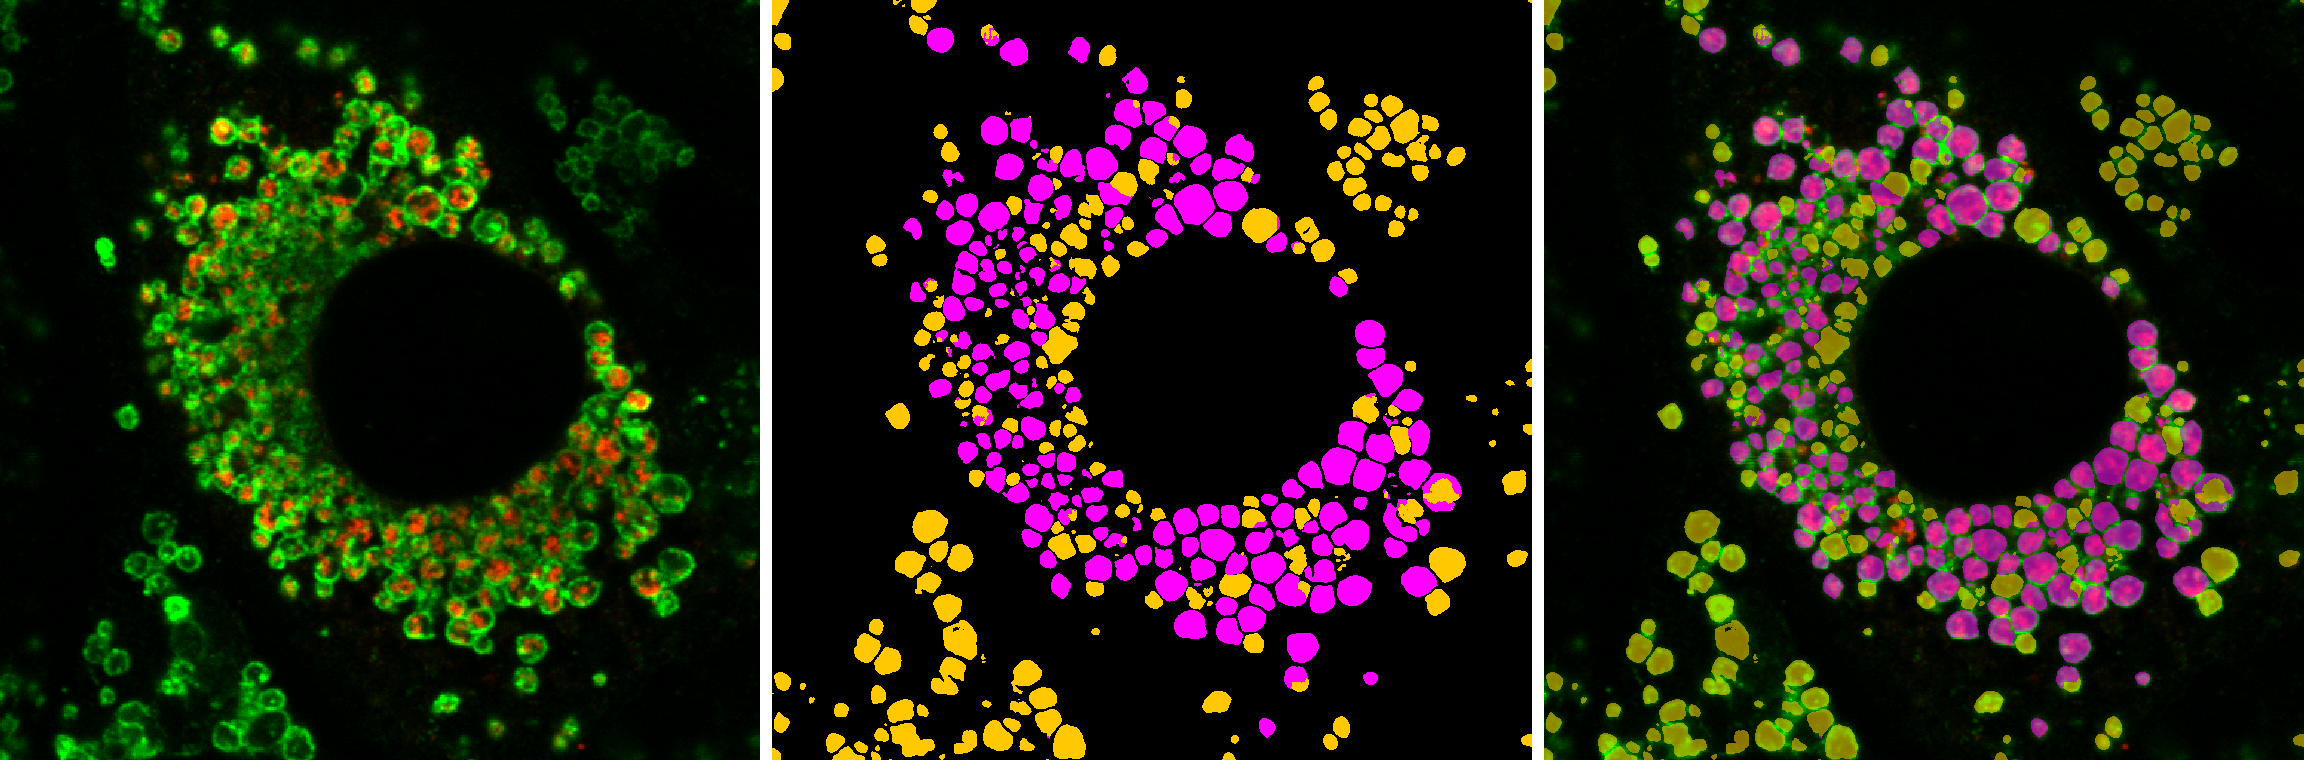
\includegraphics[width=\textwidth]{real.png}
\caption{\texttt{TEST.tif}: input (left, display-stretched), predicted classes (centre: yellow = negative, magenta = positive) and overlay (right).}\label{fig:real}
\end{figure}

Four full-size tiles ($1660{\times}1660$ inputs taken from the preprocessed, mirror-padded real image, containing all three classes) were additionally compared with the reference:

\begin{table}[h]\centering
\caption{Real-image tiles (origin in the padded frame). Max.\ score $\approx 11.5$--$13$.}
\begin{tabular}{lccc}\toprule
Origin & PyTorch f64 & PyTorch f32 & argmax equal\\\midrule
(1000,1000) & \num{3.0e-14} & \num{1.8e-05} & 100\%\\
(300,1400) & \num{3.5e-14} & \num{1.8e-05} & 100\%\\
(1900,500) & \num{2.8e-14} & \num{2.3e-05} & 100\%\\
(0,0) & \num{3.0e-14} & \num{1.6e-05} & 100\%\\\bottomrule
\end{tabular}
\end{table}

Across the 132\,$\times$\,132 outputs of these tiles, every pixel gets the same label from both implementations, so the segmentation is unaffected by the implementation.

\section{Tiling behaviour (shift equivariance)}
A U-Net with $L=7$ max-pools is translation-equivariant only for shifts that are multiples of $2^L=128$. I measured this directly on the port (shifted crops of one canvas, comparing the overlapping outputs):

\begin{center}\begin{tabular}{rcc}\toprule
Shift (px) & max.\ score difference & label agreement\\\midrule
128 / 256 & \num{7.6e-06} / \num{5.7e-06} & 100\%\\
64 & \num{5.3e-03} & 100\%\\
132 & \num{0.96} & 100\%\\
4 & \num{2.4} & 99.93\%\\\bottomrule
\end{tabular}\end{center}

Shifts by multiples of 128 are exact; others change the pooling grid and thus the scores (rarely the labels). Valid output tiles have size $4+128k$, so adjacent tiles are never 128-aligned, and a tiled run differs slightly from a single-pass run (e.g.\ $2.3\%$ of pixels on a synthetic $200{\times}230$ image tiled with 132 px against one pass). This is a property of the architecture, not of the port: the Caffe network has the same pooling layers and hence the same constraint. It does mean that exact agreement with the Caffe plugin on whole images additionally requires identical tile origins; Section~\ref{sec:caffe} shows that this is indeed the case for the default tile size of the server.

\section{Comparison with the Caffe segmentation}\label{sec:caffe}
The previous sections compare the PyTorch network with the \emph{specification} of the Caffe network. As a direct end-to-end test, \texttt{test/LQ\_TEST.tif} contains the segmentation of \texttt{TEST.tif} made with the original Caffe-based plugin ($2279{\times}2279$ labels: 0 background, 1 negative, 2 positive; it has exactly the size of the rescaled image in the previous section). I ran the server on \texttt{TEST.tif} exactly as above (default tile size 900, $3{\times}3$ tiles, CPU, float32) and compared the two label images pixel by pixel (\texttt{report/verification/compare\_caffe.py}).

\subsection{Pixel level}
\begin{table}[h]\centering
\caption{Confusion matrix of the PyTorch labels against the Caffe labels (pixels).}\label{tab:conf}
\begin{tabular}{l rrr}\toprule
 & \multicolumn{3}{c}{PyTorch}\\\cmidrule(l){2-4}
Caffe & background & negative & positive\\\midrule
background & \num[scientific-notation=false,round-mode=none]{4211607} & 13 & 50\\
negative & 16 & \num[scientific-notation=false,round-mode=none]{428889} & 6\\
positive & 31 & 2 & \num[scientific-notation=false,round-mode=none]{553227}\\\bottomrule
\end{tabular}
\end{table}

Of $\num[scientific-notation=false,round-mode=none]{5193841}$ pixels, 118 (0.0023\%) are labelled differently, i.e.\ the overall agreement is 99.9977\%. Per class, the Dice coefficient between the two segmentations is 0.99996 (negative), 0.99992 (positive) and 0.99994 (any lysosome), with the lysosome area differing by 16 px out of $982\,171$ (negative: $428\,911$ vs.\ $428\,904$ px; positive: $553\,260$ vs.\ $553\,283$ px). Only 8 of the 118 pixels change between the two lysosome classes (6 negative$\to$positive, 2 positive$\to$negative); the other 110 are lysosome/background pixels on object borders.

\begin{figure}[h]\centering
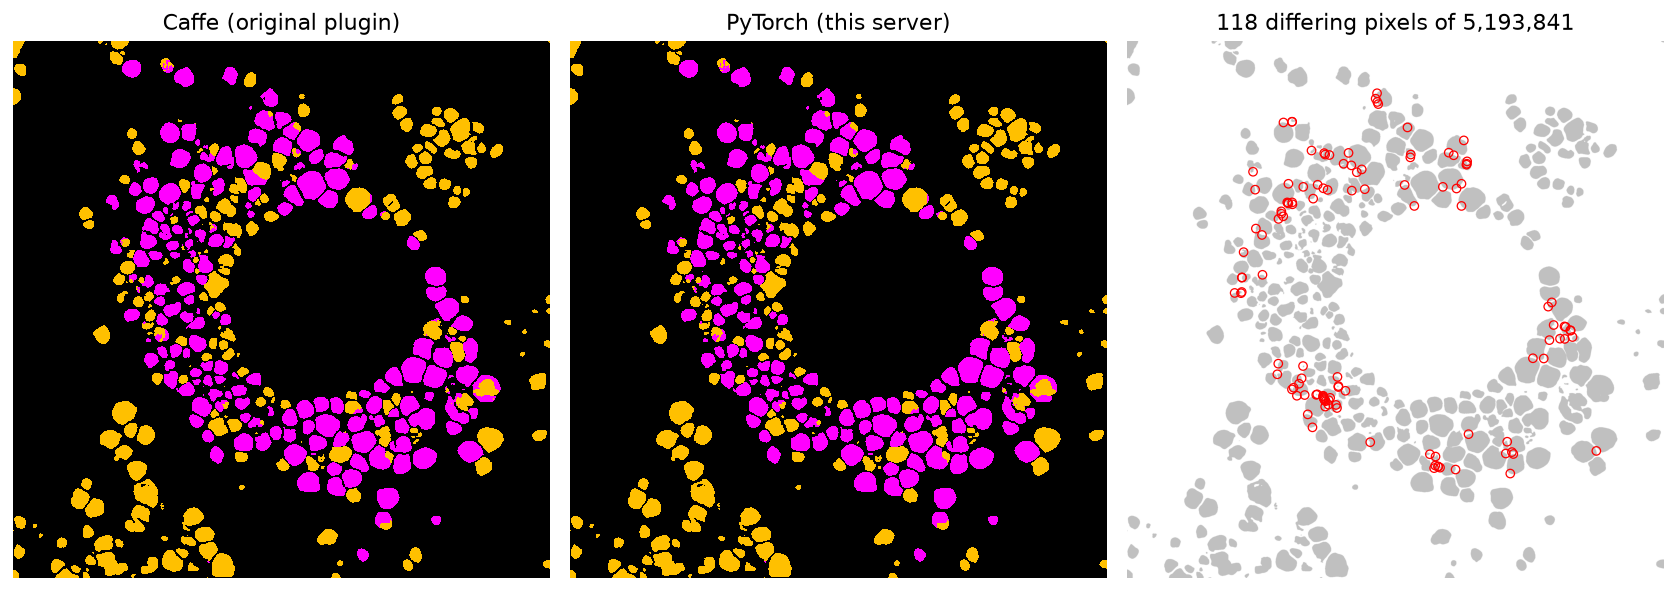
\includegraphics[width=\textwidth]{compare_overview.png}
\caption{\texttt{TEST.tif}: segmentation by the Caffe plugin (left) and by the PyTorch server (centre), yellow = negative, magenta = positive. Right: the 118 pixels (red circles, enlarged) at which they differ, over the Caffe foreground (grey). The two label images are visually indistinguishable.}\label{fig:overview}
\end{figure}

\subsection{Nature of the residual differences}
The 118 differing pixels form 115 clusters of at most 2 pixels; 95\% of them are within 2 px of an object border (Fig.~\ref{fig:zoom}), none is within 10 px of the image border, and only 5 are within 5 px of a tile edge, so they are not tiling artefacts. They occur only where the network itself is undecided: the difference between the two highest class scores is below $0.054$ at these pixels (median 0.003), against a median of 14.4 over the image (Fig.~\ref{fig:margin}); a mere 0.36\% of all pixels have a margin below 0.1. A one-pixel shift of an object border is the expected effect of any tiny numerical difference in the scores. The float32 discrepancy against the NumPy reference measured above ($\sim2\cdot10^{-5}$) is smaller than the largest score margin of the differing pixels, so rounding in the network alone may not explain all of them; the other candidates are differences in the resampling or normalisation of the input (the Java and Python implementations of the bilinear rescaling) and the different hardware and convolution algorithms of the two frameworks. I did not isolate which contributes.

\begin{figure}[h]\centering
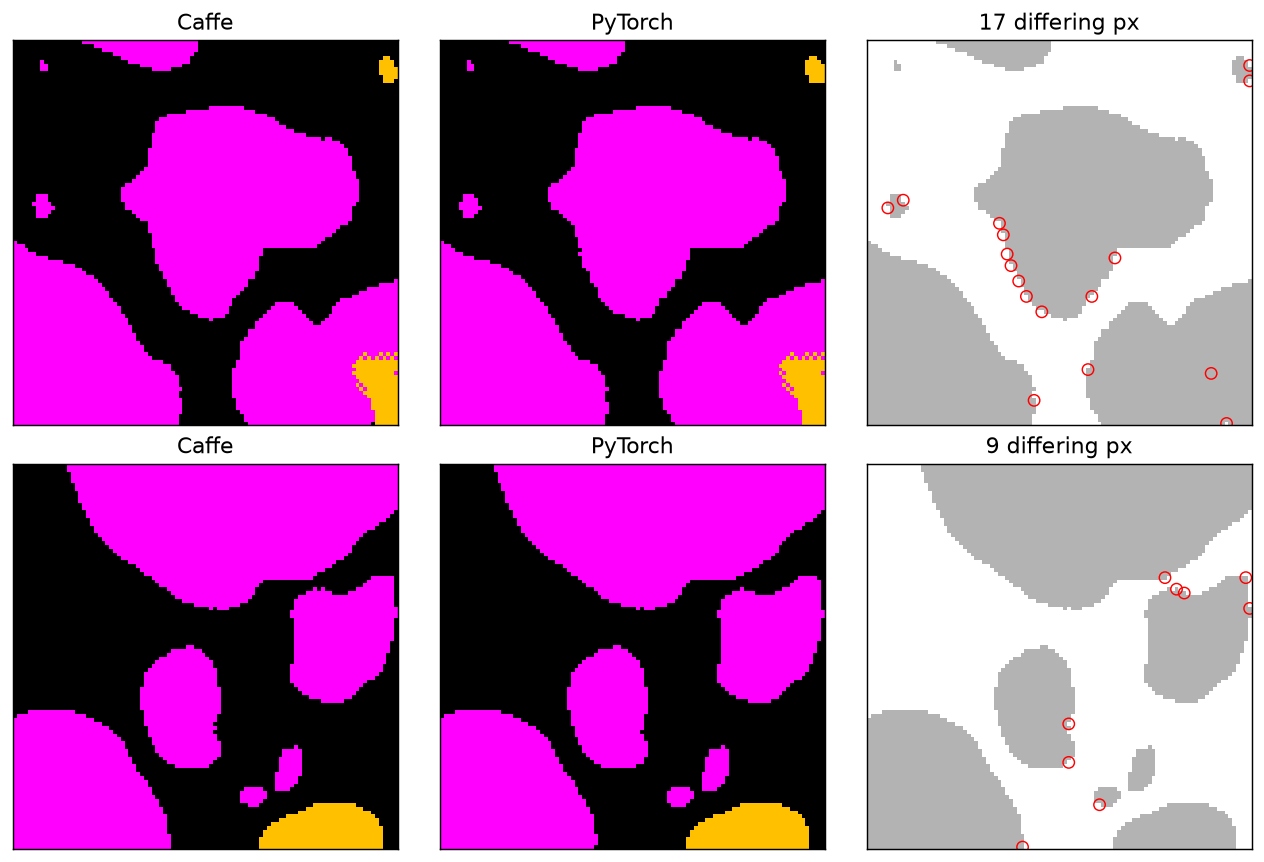
\includegraphics[width=.9\textwidth]{compare_zoom.png}
\caption{The two $100{\times}100$ px regions with most differences (17 and 9 pixels). The differing pixels (red circles, right) are single-pixel shifts of an object border.}\label{fig:zoom}
\end{figure}

\begin{figure}[h]\centering
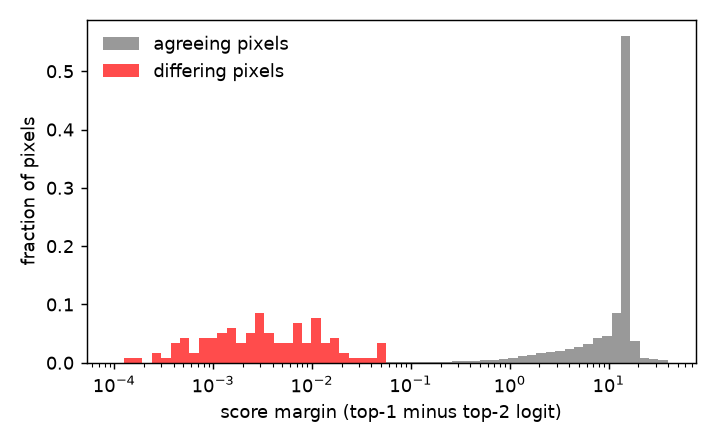
\includegraphics[width=.6\textwidth]{compare_margin.png}
\caption{Distribution of the score margin (top-1 minus top-2 class score) of the PyTorch output, for pixels labelled like Caffe (grey) and differently (red); each histogram is normalised to its own total. All differing pixels are near-ties.}\label{fig:margin}
\end{figure}

\subsection{Object level}
Counting 8-connected objects (the default of ImageJ's particle analyser), the two segmentations contain 385 vs.\ 384 lysosomes (negative 263 vs.\ 262, positive 222 vs.\ 223; Table~\ref{tab:obj}). The difference in counts comes from one-pixel specks: in the negative class, two single-pixel objects of the Caffe result are joined into one 3-pixel object by one extra PyTorch pixel; in the positive class PyTorch has one additional single-pixel object. Each Caffe object was matched to the PyTorch object with which it overlaps most: 322 of 385 are pixel-identical in both outputs and the mean intersection over union is 0.9958 (0.9990 for positive and 0.9943 for negative objects; the lowest value, 0.33, belongs to the two joined single-pixel specks; no positive object has an IoU below 0.92). These measurements do not take into account any size exclusion filtering on the objects.

\begin{table}[h]\centering
\caption{Objects (8-connected) in the Caffe and PyTorch segmentations; ``identical'': best-overlap match has IoU = 1.}\label{tab:obj}
\begin{tabular}{lrrrr}\toprule
Class & Caffe & PyTorch & identical & mean IoU\\\midrule
negative & 263 & 262 & 239 & 0.9943\\
positive & 222 & 223 & 174 & 0.9990\\
all & 385 & 384 & 322 & 0.9958\\\bottomrule
\end{tabular}
\end{table}

\subsection{Dependence on the tile size}
Because of the pooling grid (previous section), the segmentation depends on where the tiles are placed. I repeated the run with other tile sizes and compared each with the Caffe result:

\begin{center}\begin{tabular}{rrrr}\toprule
Tile (px) & Tiles & Pixels differing from Caffe & Fraction\\\midrule
388 & 36 & \num[scientific-notation=false,round-mode=none]{90644} & 1.75\%\\
516 & 25 & \num[scientific-notation=false,round-mode=none]{79470} & 1.53\%\\
\textbf{900} & 9 & \textbf{118} & \textbf{0.0023\%}\\
1156 & 4 & \num[scientific-notation=false,round-mode=none]{35813} & 0.69\%\\\bottomrule
\end{tabular}\end{center}

Only the default tile size of 900 px reproduces the Caffe result; the others differ by roughly 300 to 800 times more pixels. The original plugin therefore must have used the same tile layout (output tiles of 900 px starting at multiples of 900 with mirror padding) as \texttt{predict.py}. Conversely, the tile size of the server is not free if results are to be comparable with earlier Caffe-based analyses: it changes up to 1.7\% of the pixels of this image, more than the 0.002\% attributable to the port itself. Whether other tile sizes were in use in the original plugin for other image sizes was not investigated.

\section{Conclusion}
The PyTorch model is the Caffe model: identical architecture (38 parametrised layers, 37 LeakyReLU(0.1) activations, 7 poolings, 7 deconvolutions, centre-cropped skip connections, $-0.5$ input offset), bit-identical weights, and a forward pass that matches an independent execution of the original \texttt{prototxt} to machine precision in float64 and to $\sim10^{-6}$ relative in float32, giving identical segmentations on real data. Against the output of the original Caffe plugin on a real image, the full PyTorch pipeline reproduces 99.9977\% of the pixels (Dice $>0.9999$ for both classes, 322 of 385 lysosomes pixel-identical, the others differing by a few border pixels); the 118 differing pixels are single-pixel border shifts at near-ties of the class scores. This holds for the default tile size of 900 px, which the original evidently used; other tile sizes change about 1\% of the pixels of this image. When the exclusion filter of the ImageJ plugin is applied (objects smaller than \SI{0.53}{\micro m\squared}, i.e.\ 848 px at the model pixel size of \SI{0.025}{\micro m}), the two segmentations give identical counts: 295 lysosomes in total, of which 149 negative and 146 positive. The filter removes the single-pixel objects responsible for the unfiltered difference of one object per class, and the retained objects differ in area by at most 9 px (0.4\%). The differences between the two implementations are therefore confined to single border pixels and do not affect the quantities reported by LysoQuant on this image, so that the PyTorch implementation can replace the Caffe one.
\end{document}
